\documentclass{beamer}

\usepackage[T1]{fontenc}   % required for luximono!
\usepackage{lmodern}
\usepackage[scaled=0.8]{luximono}  % typewriter font with bold face

% To install the luximono font files:
% getnonfreefonts-sys --all        or
% getnonfreefonts-sys luximono
%
% when there are trouble you might need to:
% - Create /etc/texmf/updmap.d/99local-luximono.cfg
%   containing the single line: Map ul9.map
% - Run update-updmap followed by mktexlsr and updmap-sys
%
% This commands must be executed as root with a root environment
% (i.e. run "sudo su" and then execute the commands in the root
% shell, don't just prefix the commands with "sudo").

% formats the text accourding the set language
\usepackage[english]{babel}
\usepackage{amsmath}
\usepackage{multirow}
\usepackage{booktabs}
\usepackage{listings}
\usepackage{setspace}
\usepackage{skull}
\usepackage{units}

\usepackage{tikz}
\usetikzlibrary{calc}
\usetikzlibrary{arrows}
\usetikzlibrary{scopes}
\usetikzlibrary{through}
\usetikzlibrary{shapes.geometric}

\lstset{basicstyle=\ttfamily}

\def\B#1{{\tt\textbackslash{}#1}}
\def\C#1{\lstinline[language=C++]{#1}}
\def\V#1{\lstinline[language=Verilog]{#1}}

\lstdefinelanguage{liberty}{
	morecomment=[s]{/*}{*/},
	morekeywords={library,cell,area,pin,direction,function,clocked_on,next_state,clock,ff},
	morestring=[b]",
}

\lstdefinelanguage{rtlil}{
	morecomment=[l]{\#},
	morekeywords={module,attribute,parameter,wire,memory,auto,width,offset,size,input,output,inout,cell,connect,switch,case,assign,sync,low,high,posedge,negedge,edge,always,update,process,end},
	morestring=[b]",
}

\newenvironment{boxalertenv}{\begin{altenv}%
{\usebeamertemplate{alerted text begin}\usebeamercolor[fg]{alerted text}\usebeamerfont{alerted text}\setlength{\fboxsep}{1pt}\colorbox{bg}}
{\usebeamertemplate{alerted text end}}{\color{.}}{}}{\end{altenv}}

\newcommand<>{\boxalert}[1]{{%
\begin{boxalertenv}#2{#1}\end{boxalertenv}%
}}

\title{Yosys Open SYnthesis Suite}
\author{Clifford Wolf}
\institute{http://www.clifford.at/}

\usetheme{Madrid}
\usecolortheme{seagull}
\beamertemplatenavigationsymbolsempty

\definecolor{YosysGreen}{RGB}{85,136,102}
\definecolor{MyBlue}{RGB}{85,130,180}

\setbeamercolor{title}{fg=black,bg=YosysGreen!70}
\setbeamercolor{titlelike}{fg=black,bg=YosysGreen!70}
\setbeamercolor{frametitle}{fg=black,bg=YosysGreen!70}
\setbeamercolor{block title}{fg=black,bg=YosysGreen!70}
\setbeamercolor{item projected}{fg=black,bg=YosysGreen}

\begin{document}

\begin{frame}
\titlepage
\end{frame}

\setcounter{section}{-2}

\section{Abstract}
\begin{frame}{Abstract}
Yosys is the first full-featured open source software for Verilog HDL
synthesis. It supports most of Verilog-2005 and is well tested with
real-world designs from the ASIC and FPGA world.

\bigskip
Learn how to use Yosys to create your own custom synthesis flows and discover
why open source HDL synthesis is important for researchers, hobbyists,
educators and engineers alike.

\bigskip
This presentation covers basic concepts of Yosys, creating simple synthesis
scripts, creating synthesis scripts for advanced applications, creating Yosys
scripts for non-synthesis applications (such as formal equivialence checking)
and writing extensions to Yosys using the C++ API.
\end{frame}

\section{Outline}
\begin{frame}{Outline}
Yosys is an Open Source Verilog synthesis tool, and more.

\bigskip
Outline of this presentation:
\begin{itemize}
\item Introduction to the field and Yosys
\item Yosys by example: synthesis
\item Yosys by example: advanced synthesis
\item Yosys by example: beyond synthesis
\item Programming Yosys extensions
\end{itemize}
\end{frame}


\section{Introduction}

\begin{frame}
\sectionpage
\end{frame}

%%%%%%%%%%%%%%%%%%%%%%%%%%%%%%%%%%%%%%%%%%%%%%%%%%%%%%%%%%%%%%%%%%%%%%%%%%%%%

\subsection{Representations of (digital) Circuits}

\begin{frame}[t]{\subsecname}
\begin{itemize}
	\item Graphical
		\begin{itemize}
			\item \alert<1>{Schematic Diagram}
			\item \alert<2>{Physical Layout}
		\end{itemize}
	\bigskip
	\item Non-graphical
		\begin{itemize}
			\item \alert<3>{Netlists}
			\item \alert<4>{Hardware Description Languages (HDLs)}
		\end{itemize}
\end{itemize}
\bigskip
\begin{block}{Definition:
\only<1>{Schematic Diagram}%
\only<2>{Physical Layout}%
\only<3>{Netlists}%
\only<4>{Hardware Description Languages (HDLs)}}
\only<1>{
	Graphical representation of the circtuit topology. Circuit elements
	are represented by symbols and electrical connections by lines. The gometric
	layout is for readability only.
}%
\only<2>{
	The actual physical geometry of the device (PCB or ASIC manufracturing masks).
	This is the final product of the design process.
}%
\only<3>{
	A list of circuit elements and a list of connections. This is the raw circuit
	topology.
}%
\only<4>{
	Computer languages (like programming languages) that can be used to describe
	circuits. HDLs are much more powerful in describing huge circuits than
	schematic diagrams.
}%
\end{block}
\end{frame}

%%%%%%%%%%%%%%%%%%%%%%%%%%%%%%%%%%%%%%%%%%%%%%%%%%%%%%%%%%%%%%%%%%%%%%%%%%%%%

\subsection{Levels of Abstraction for Digital Circuits}

\begin{frame}[t]{\subsecname}
\begin{itemize}
	\item \alert<1>{System Level}
	\item \alert<2>{High Level}
	\item \alert<3>{Behavioral Level}
	\item \alert<4>{Register-Transfer Level (RTL)}
	\item \alert<5>{Logical Gate Level}
	\item \alert<6>{Physical Gate Level}
	\item \alert<7>{Switch Level}
\end{itemize}
\bigskip
\begin{block}{Definition:
\only<1>{System Level}%
\only<2>{High Level}%
\only<3>{Behavioral Level}%
\only<4>{Register-Transfer Level (RTL)}%
\only<5>{Logical Gate Level}%
\only<6>{Physical Gate Level}%
\only<7>{Switch Level}}
\only<1>{
	Overall view of the circuit: E.g. block-diagrams or instruction-set architecture descriptions
}%
\only<2>{
	Functional implementation of circuit in high-level programming language (C, C++, SystemC, Matlab, Python, etc.).
}%
\only<3>{
	Cycle-accurate description of circuit in hardware description language (Verilog, VHDL, etc.).
}%
\only<4>{
	List of registers (flip-flops) and logic functions that calculate the next state from the previous one. Usually
	a netlist utilizing high-level cells such as adders, multiplieres, multiplexer, etc.
}%
\only<5>{
	Netlist of single-bit registers and basic logic gates (such as AND, OR,
	NOT, etc.). Popular form: And-Inverter-Graphs (AIGs) with pairs of primary
	inputs and outputs for each register bit.
}%
\only<6>{
	Netlist of cells that actually are available on the target architecture
	(such as CMOS gates in an ASCI or LUTs in an FPGA). Optimized for
	area and/or and/or speed (static timing or number of logic levels).
}%
\only<7>{
	Netlist of individual transistors.
}%
\end{block}
\end{frame}

%%%%%%%%%%%%%%%%%%%%%%%%%%%%%%%%%%%%%%%%%%%%%%%%%%%%%%%%%%%%%%%%%%%%%%%%%%%%%

\subsection{Digital Circuit Synthesis}

\begin{frame}{\subsecname}
	Synthesis Tools (such as Yosys) can transform HDL code to circuits:

	\bigskip
	\begin{center}
	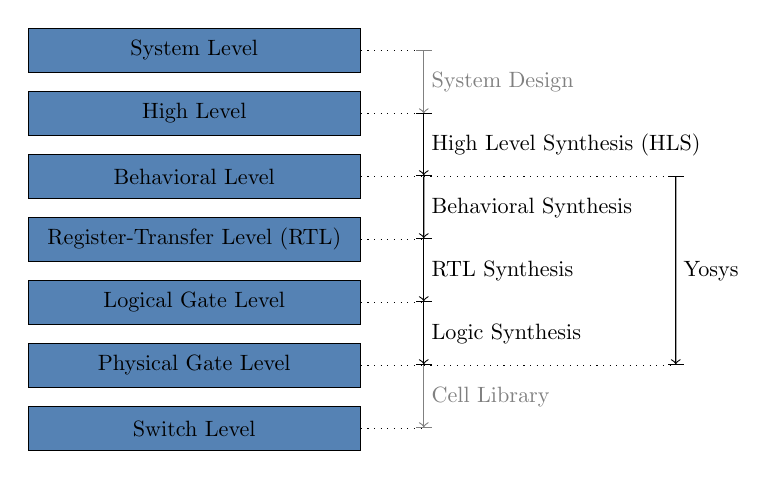
\begin{tikzpicture}[scale=0.8, every node/.style={transform shape}]
			\tikzstyle{lvl} = [draw, fill=MyBlue, rectangle, minimum height=2em, minimum width=15em]
			\node[lvl] (sys) {System Level};
			\node[lvl] (hl) [below of=sys] {High Level};
			\node[lvl] (beh) [below of=hl] {Behavioral Level};
			\node[lvl] (rtl) [below of=beh] {Register-Transfer Level (RTL)};
			\node[lvl] (lg) [below of=rtl] {Logical Gate Level};
			\node[lvl] (pg) [below of=lg] {Physical Gate Level};
			\node[lvl] (sw) [below of=pg] {Switch Level};

			\draw[dotted] (sys.east)  -- ++(1,0) coordinate (sysx);
			\draw[dotted] (hl.east)  -- ++(1,0) coordinate (hlx);
			\draw[dotted] (beh.east) -- ++(1,0) coordinate (behx);
			\draw[dotted] (rtl.east) -- ++(1,0) coordinate (rtlx);
			\draw[dotted] (lg.east)  -- ++(1,0) coordinate (lgx);
			\draw[dotted] (pg.east)  -- ++(1,0) coordinate (pgx);
			\draw[dotted] (sw.east)  -- ++(1,0) coordinate (swx);

			\draw[gray,|->] (sysx) -- node[right] {System Design} (hlx);
			\draw[|->|] (hlx) -- node[right] {High Level Synthesis (HLS)} (behx);
			\draw[->|] (behx) -- node[right] {Behavioral Synthesis} (rtlx);
			\draw[->|] (rtlx) -- node[right] {RTL Synthesis} (lgx);
			\draw[->|] (lgx) -- node[right] {Logic Synthesis} (pgx);
			\draw[gray,->|] (pgx) -- node[right] {Cell Library} (swx);

			\draw[dotted] (behx) -- ++(4,0) coordinate (a);
			\draw[dotted] (pgx) -- ++(4,0) coordinate (b);
			\draw[|->|] (a) -- node[right] {Yosys} (b);
	\end{tikzpicture}
	\end{center}
\end{frame}

%%%%%%%%%%%%%%%%%%%%%%%%%%%%%%%%%%%%%%%%%%%%%%%%%%%%%%%%%%%%%%%%%%%%%%%%%%%%%

\subsection{What Yosys can and can't do}

\begin{frame}{\subsecname}

Things Yosys can do:
\begin{itemize}
\item Read and process (most of) modern Verilog-2005 code.
\item Perform all kinds of operations on netlist (RTL, Logic, Gate).
\item Perform logic optimiziations and gate mapping with ABC\footnote[frame]{\url{http://www.eecs.berkeley.edu/~alanmi/abc/}}.
\end{itemize}

\bigskip
Things Yosys can't do:
\begin{itemize}
\item Process high-level languages such as C/C++/SystemC.
\item Create physical layouts (place\&route).
\end{itemize}

\bigskip
A typical flow combines Yosys with with a low-level implementation tool, such
as Qflow\footnote[frame]{\url{http://opencircuitdesign.com/qflow/}} for ASIC designs.

\end{frame}

%%%%%%%%%%%%%%%%%%%%%%%%%%%%%%%%%%%%%%%%%%%%%%%%%%%%%%%%%%%%%%%%%%%%%%%%%%%%%

\subsection{Yosys Data- and Control-Flow}

\begin{frame}{\subsecname}
	A (usually short) synthesis script controlls Yosys.

	This scripts contain three types of commands:
	\begin{itemize}
	\item {\bf Frontends}, that read input files (usually Verilog).
	\item {\bf Passes}, that perform transformation on the design in memory.
	\item {\bf Backends}, that write the design in memory to a file (various formats are available, e.g. Verilog, BLIF, EDIF, SPICE, BTOR, etc.).
	\end{itemize}

	\bigskip
	\begin{center}
	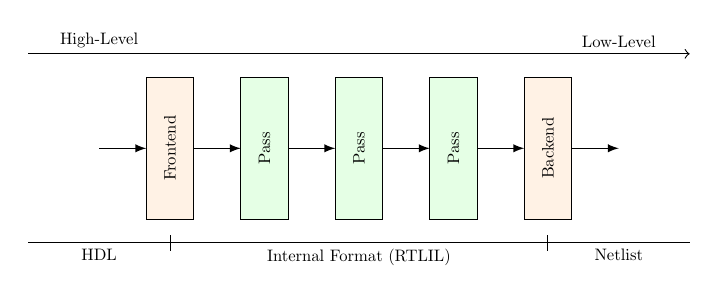
\begin{tikzpicture}[scale=0.6, every node/.style={transform shape}]
		\path (-1.5,3) coordinate (cursor);
		\draw[-latex] ($ (cursor) + (0,-1.5) $) -- ++(1,0);
		\draw[fill=orange!10] ($ (cursor) + (1,-3) $) rectangle node[rotate=90] {Frontend} ++(1,3) coordinate (cursor);
		\draw[-latex] ($ (cursor) + (0,-1.5) $) -- ++(1,0);
		\draw[fill=green!10] ($ (cursor) + (1,-3) $) rectangle node[rotate=90] {Pass} ++(1,3) coordinate (cursor);
		\draw[-latex] ($ (cursor) + (0,-1.5) $) -- ++(1,0);
		\draw[fill=green!10] ($ (cursor) + (1,-3) $) rectangle node[rotate=90] {Pass} ++(1,3) coordinate (cursor);
		\draw[-latex] ($ (cursor) + (0,-1.5) $) -- ++(1,0);
		\draw[fill=green!10] ($ (cursor) + (1,-3) $) rectangle node[rotate=90] {Pass} ++(1,3) coordinate (cursor);
		\draw[-latex] ($ (cursor) + (0,-1.5) $) -- ++(1,0);
		\draw[fill=orange!10] ($ (cursor) + (1,-3) $) rectangle node[rotate=90] {Backend} ++(1,3) coordinate (cursor);
		\draw[-latex] ($ (cursor) + (0,-1.5) $) -- ++(1,0);

		\path (-3,-0.5) coordinate (cursor);
		\draw (cursor) -- node[below] {HDL} ++(3,0) coordinate (cursor);
		\draw[|-|] (cursor) -- node[below] {Internal Format (RTLIL)} ++(8,0) coordinate (cursor);
		\draw (cursor) -- node[below] {Netlist} ++(3,0);

		\path (-3,3.5) coordinate (cursor);
		\draw[-] (cursor) -- node[above] {High-Level} ++(3,0) coordinate (cursor);
		\draw[-] (cursor) -- ++(8,0) coordinate (cursor);
		\draw[->] (cursor) -- node[above] {Low-Level} ++(3,0);
	\end{tikzpicture}
	\end{center}
\end{frame}

%%%%%%%%%%%%%%%%%%%%%%%%%%%%%%%%%%%%%%%%%%%%%%%%%%%%%%%%%%%%%%%%%%%%%%%%%%%%%

\subsection{Program Components and Data Formats}

\begin{frame}{\subsecname}
	\begin{center}
	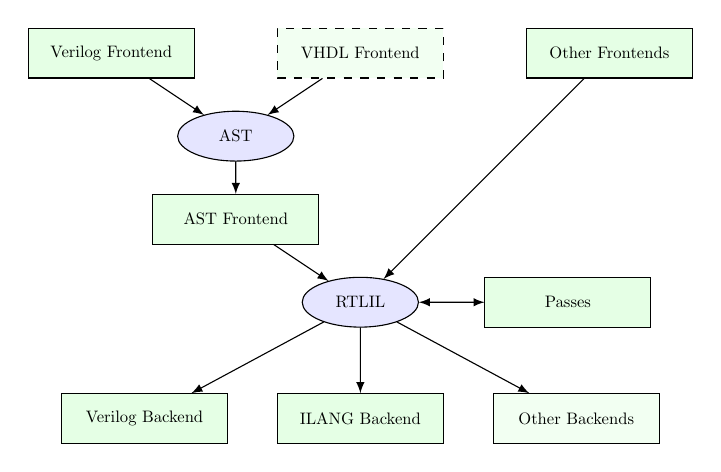
\begin{tikzpicture}[scale=0.6, every node/.style={transform shape}]
		\tikzstyle{process} = [draw, fill=green!10, rectangle, minimum height=3em, minimum width=10em, node distance=15em]
		\tikzstyle{data} = [draw, fill=blue!10, ellipse, minimum height=3em, minimum width=7em, node distance=15em]
		\node[process] (vlog) {Verilog Frontend};
		\node[process, dashed, fill=green!5] (vhdl) [right of=vlog] {VHDL Frontend};
		\node[process] (ilang) [right of=vhdl] {Other Frontends};
		\node[data] (ast) [below of=vlog, node distance=5em, xshift=7.5em] {AST};
		\node[process] (astfe) [below of=ast, node distance=5em] {AST Frontend};
		\node[data] (rtlil) [below of=astfe, node distance=5em, xshift=7.5em] {RTLIL};
		\node[process] (pass) [right of=rtlil, node distance=5em, xshift=7.5em] {Passes};
		\node[process] (vlbe) [below of=rtlil, node distance=7em, xshift=-13em] {Verilog Backend};
		\node[process] (ilangbe) [below of=rtlil, node distance=7em, xshift=0em] {ILANG Backend};
		\node[process, fill=green!5] (otherbe) [below of=rtlil, node distance=7em, xshift=+13em] {Other Backends};

		\draw[-latex] (vlog) -- (ast);
		\draw[-latex] (vhdl) -- (ast);
		\draw[-latex] (ast) -- (astfe);
		\draw[-latex] (astfe) -- (rtlil);
		\draw[-latex] (ilang) -- (rtlil);
		\draw[latex-latex] (rtlil) -- (pass);
		\draw[-latex] (rtlil) -- (vlbe);
		\draw[-latex] (rtlil) -- (ilangbe);
		\draw[-latex] (rtlil) -- (otherbe);
	\end{tikzpicture}
	\end{center}
\end{frame}

%%%%%%%%%%%%%%%%%%%%%%%%%%%%%%%%%%%%%%%%%%%%%%%%%%%%%%%%%%%%%%%%%%%%%%%%%%%%%

\subsection{Example Problem}

\begin{frame}[fragile]{\subsecname{} -- Verilog Source: \tt counter.v}
\lstinputlisting[xleftmargin=1cm, language=Verilog]{PRESENTATION_Intro/counter.v}
\end{frame}

\begin{frame}[fragile]{\subsecname{} -- Cell Library: \tt mycells.lib}
\begin{columns}
\column[t]{5cm}
\lstinputlisting[basicstyle=\ttfamily\fontsize{8pt}{10pt}\selectfont, language=liberty, lastline=20]{PRESENTATION_Intro/mycells.lib}
\column[t]{5cm}
\lstinputlisting[basicstyle=\ttfamily\fontsize{8pt}{10pt}\selectfont, language=liberty, firstline=21]{PRESENTATION_Intro/mycells.lib}
\end{columns}
\end{frame}

%%%%%%%%%%%%%%%%%%%%%%%%%%%%%%%%%%%%%%%%%%%%%%%%%%%%%%%%%%%%%%%%%%%%%%%%%%%%%

\subsection{Example Synthesis Script}

\begin{frame}[t]{\subsecname}

\setbeamercolor{alerted text}{fg=white,bg=red}

\begin{minipage}[t]{6cm}
\tt\scriptsize
\# read design\\
\boxalert<1>{read\_verilog counter.v}\\
\boxalert<2>{hierarchy -check -top counter}

\medskip
\# the high-level stuff\\
\boxalert<3>{proc}; \boxalert<4>{opt}; \boxalert<5>{memory}; \boxalert<6>{opt}; \boxalert<7>{fsm}; \boxalert<8>{opt}

\medskip
\# mapping to internal cell library\\
\boxalert<9>{techmap}; \boxalert<10>{opt}

\bigskip
\it continued\dots
\end{minipage}
\begin{minipage}[t]{5cm}
\tt\scriptsize
\# mapping flip-flops to mycells.lib\\
\boxalert<11>{dfflibmap -liberty mycells.lib}

\medskip
\# mapping logic to mycells.lib\\
\boxalert<12>{abc -liberty mycells.lib}

\medskip
\# cleanup\\
\boxalert<13>{clean}

\medskip
\# write synthesized design\\
\boxalert<14>{write\_verilog synth.v}
\end{minipage}

\vskip1cm

\begin{block}{Command: \tt
\only<1>{read\_verilog counter.v}%
\only<2>{hierarchy -check -top counter}%
\only<3>{proc}%
\only<4>{opt}%
\only<5>{memory}%
\only<6>{opt}%
\only<7>{fsm}%
\only<8>{opt}%
\only<9>{techmap}%
\only<10>{opt}%
\only<11>{dfflibmap -liberty mycells.lib}%
\only<12>{abc -liberty mycells.lib}%
\only<13>{clean}%
\only<14>{write\_verilog synth.v}}
\only<1>{
	Read Verilog source file and convert to internal representation.
}%
\only<2>{
	Elaborate the design hierarchy. Should alsways be the first
	command after reading the design.
}%
\only<3>{
	Convert ``processes'' (the internal representation of behavioral
	Verilog code) into multiplexers and registers.
}%
\only<4>{
	Perform some basic optimizations and cleanups.
}%
\only<5>{
	Analyze memories and create circuits to implement them.
}%
\only<6>{
	Perform some basic optimizations and cleanups.
}%
\only<7>{
	Analyze and optimize finite state machines.
}%
\only<8>{
	Perform some basic optimizations and cleanups.
}%
\only<9>{
	Map coarse-grain RTL cells (adders, etc.) to fine-grain
	logic gates (AND, OR, NOT, etc.).
}%
\only<10>{
	Perform some basic optimizations and cleanups.
}%
\only<11>{
	Map registers to available hardware flip-flops.
}%
\only<12>{
	Map logix to available hardware gates.
}%
\only<13>{
	Clean up the design (just the last step of {\tt opt}).
}%
\only<14>{
	Write final synthesis result to output file.
}%
\end{block}

\end{frame}

%%%%%%%%%%%%%%%%%%%%%%%%%%%%%%%%%%%%%%%%%%%%%%%%%%%%%%%%%%%%%%%%%%%%%%%%%%%%%

\subsection{Running the Synthesis Script}

\begin{frame}[t, fragile]{\subsecname{} -- Step 1/4}
\begin{verbatim}
read_verilog counter.v
hierarchy -check -top counter
\end{verbatim}

\vfill
\includegraphics[width=\linewidth,trim=0 0cm 0 0cm]{PRESENTATION_Intro/counter_00.pdf}
\end{frame}

\begin{frame}[t, fragile]{\subsecname{} -- Step 2/4}
\begin{verbatim}
proc; opt; memory; opt; fsm; opt
\end{verbatim}

\vfill
\includegraphics[width=\linewidth,trim=0 0cm 0 0cm]{PRESENTATION_Intro/counter_01.pdf}
\end{frame}

\begin{frame}[t, fragile]{\subsecname{} -- Step 3/4}
\begin{verbatim}
techmap; opt
\end{verbatim}

\vfill
\includegraphics[width=\linewidth,trim=0 0cm 0 0cm]{PRESENTATION_Intro/counter_02.pdf}
\end{frame}

\begin{frame}[t, fragile]{\subsecname{} -- Step 4/4}
\begin{verbatim}
dfflibmap -liberty mycells.lib
abc -liberty mycells.lib
clean
\end{verbatim}

\vfill
\includegraphics[width=\linewidth,trim=0 0cm 0 0cm]{PRESENTATION_Intro/counter_03.pdf}
\end{frame}

%%%%%%%%%%%%%%%%%%%%%%%%%%%%%%%%%%%%%%%%%%%%%%%%%%%%%%%%%%%%%%%%%%%%%%%%%%%%%

\subsection{Yosys Commands}

\begin{frame}[fragile]{\subsecname{} 1/3 \hspace{0pt plus 1 filll} (excerpt)}
Command reference:
\begin{itemize}
\item Use ``{\tt help}'' for a command list and ``{\tt help \it command}'' for details.
\item Or run ``{\tt yosys -H}'' and ``{\tt yosys -h \it command}''.
\item Or go to \url{http://www.clifford.at/yosys/documentation.html}.
\end{itemize}

\bigskip
Commands for design navigation and investigation:
\begin{lstlisting}[xleftmargin=1cm, basicstyle=\ttfamily\fontsize{8pt}{10pt}\selectfont]
    cd                   a shortcut for 'select -module <name>'
    ls                   list modules or objects in modules
    dump                 print parts of the design in ilang format
    show                 generate schematics using graphviz
    select               modify and view the list of selected objects
\end{lstlisting}

\bigskip
Commands for executing scripts or entering interactive mode:
\begin{lstlisting}[xleftmargin=1cm, basicstyle=\ttfamily\fontsize{8pt}{10pt}\selectfont]
    shell                enter interactive command mode
    history              show last interactive commands
    script               execute commands from script file
    tcl                  execute a TCL script file
\end{lstlisting}
\end{frame}

\begin{frame}[fragile]{\subsecname{} 2/3 \hspace{0pt plus 1 filll} (excerpt)}
Commands for reading and elaborating the design:
\begin{lstlisting}[xleftmargin=1cm, basicstyle=\ttfamily\fontsize{8pt}{10pt}\selectfont]
    read_ilang           read modules from ilang file
    read_verilog         read modules from verilog file
    hierarchy            check, expand and clean up design hierarchy
\end{lstlisting}

\bigskip
Commands for high-level synthesis:
\begin{lstlisting}[xleftmargin=1cm, basicstyle=\ttfamily\fontsize{8pt}{10pt}\selectfont]
    proc                 translate processes to netlists
    fsm                  extract and optimize finite state machines
    memory               translate memories to basic cells
    opt                  perform simple optimizations
\end{lstlisting}

\bigskip
Commands for technology mapping:
\begin{lstlisting}[xleftmargin=1cm, basicstyle=\ttfamily\fontsize{8pt}{10pt}\selectfont]
    techmap              simple technology mapper
    abc                  use ABC for technology mapping
    dfflibmap            technology mapping of flip-flops
    hilomap              technology mapping of constant hi- and/or lo-drivers
    iopadmap             technology mapping of i/o pads (or buffers)
    flatten              flatten design
\end{lstlisting}
\end{frame}

\begin{frame}[fragile]{\subsecname{} 3/3 \hspace{0pt plus 1 filll} (excerpt)}
Commands for writing the results:
\begin{lstlisting}[xleftmargin=1cm, basicstyle=\ttfamily\fontsize{8pt}{10pt}\selectfont]
    write_blif           write design to BLIF file
    write_btor           write design to BTOR file
    write_edif           write design to EDIF netlist file
    write_ilang          write design to ilang file
    write_spice          write design to SPICE netlist file
    write_verilog        write design to verilog file
\end{lstlisting}

\bigskip
Script-Commands for standard synthesis tasks:
\begin{lstlisting}[xleftmargin=1cm, basicstyle=\ttfamily\fontsize{8pt}{10pt}\selectfont]
    synth_xilinx         synthesis for Xilinx FPGAs
\end{lstlisting}

\bigskip
... and many many more.
\end{frame}

%%%%%%%%%%%%%%%%%%%%%%%%%%%%%%%%%%%%%%%%%%%%%%%%%%%%%%%%%%%%%%%%%%%%%%%%%%%%%

\subsection{More Verilog Examples}

\begin{frame}[fragile]{\subsecname{} 1/3}
\begin{lstlisting}[xleftmargin=1cm, basicstyle=\ttfamily\fontsize{8pt}{10pt}\selectfont, language=Verilog]
module detectprime(a, y);
    input [4:0] a;
    output y;

    integer i, j;
    reg [31:0] lut;

    initial begin
        for (i = 0; i < 32; i = i+1) begin
            lut[i] = i > 1;
            for (j = 2; j*j <= i; j = j+1)
                if (i % j == 0)
                    lut[i] = 0;
        end
    end

    assign y = lut[a];
endmodule
\end{lstlisting}
\end{frame}

\begin{frame}[fragile]{\subsecname{} 2/3}
\begin{lstlisting}[xleftmargin=1cm, basicstyle=\ttfamily\fontsize{8pt}{10pt}\selectfont, language=Verilog]
module carryadd(a, b, y);
    parameter WIDTH = 8;
    input [WIDTH-1:0] a, b;
    output [WIDTH-1:0] y;

    genvar i;
    generate
        for (i = 0; i < WIDTH; i = i+1) begin:STAGE
            wire IN1 = a[i], IN2 = b[i];
            wire C, Y;
            if (i == 0)
                assign C = IN1 & IN2, Y = IN1 ^ IN2;
            else
                assign C = (IN1 & IN2) | ((IN1 | IN2) & STAGE[i-1].C),
                       Y = IN1 ^ IN2 ^ STAGE[i-1].C;
            assign y[i] = Y;
        end
    endgenerate
endmodule
\end{lstlisting}
\end{frame}

\begin{frame}[fragile]{\subsecname{} 3/3}
\begin{lstlisting}[xleftmargin=1cm, basicstyle=\ttfamily\fontsize{7pt}{8.5pt}\selectfont, language=Verilog]
module cam(clk, wr_enable, wr_addr, wr_data, rd_data, rd_addr, rd_match);
    parameter WIDTH = 8;
    parameter DEPTH = 16;
    localparam ADDR_BITS = $clog2(DEPTH);

    input clk, wr_enable;
    input [ADDR_BITS-1:0] wr_addr;
    input [WIDTH-1:0] wr_data, rd_data;
    output reg [ADDR_BITS-1:0] rd_addr;
    output reg rd_match;

    integer i;
    reg [WIDTH-1:0] mem [0:DEPTH-1];

    always @(posedge clk) begin
        rd_addr <= 'bx;
        rd_match <= 0;
        for (i = 0; i < DEPTH; i = i+1)
            if (mem[i] == rd_data) begin
                rd_addr <= i;
                rd_match <= 1;
            end
        if (wr_enable)
            mem[wr_addr] <= wr_data;
    end
endmodule
\end{lstlisting}
\end{frame}

\subsection{Verification}

\begin{frame}{\subsecname}
Contiously checking the correctness of Yosys and making sure that new features
do not break old ones is a high priority in Yosys.

\bigskip
There are two external test suites build for Yosys: VlogHammer and yosys-bigsim
(see next slides)

\bigskip
In addition to that, yosys comes with $\approx\!200$ test cases used in ``{\tt make test}''.

\bigskip
A debug build of Yosys also contains a lot of asserts and checks the integrity of
the internal state after each command.
\end{frame}

\begin{frame}[fragile]{\subsecname{} -- VlogHammer}
VlogHammer is a Verilog regression test suite developed to test the different
subsystems in Yosys by comparing them to each other and the implementations
generated by some proprietary tools (Xilinx Vivado, Xilinx XST, Altera Quartus II, ...).

\bigskip
Yosys Subsystems tested: Verilog frontend, const folding, const eval, technology mapping,
simulation models, SAT models.

\bigskip
Thousands of auto-generated test cases containing code such as:
\begin{lstlisting}[xleftmargin=1cm, basicstyle=\ttfamily\fontsize{8pt}{10pt}\selectfont, language=Verilog]
assign y9 = $signed(((+$signed((^(6'd2 ** a2))))<$unsigned($unsigned(((+a3))))));
assign y10 = (-((+((+{2{(~^p13)}})))^~(!{{b5,b1,a0},(a1&p12),(a4+a3)})));
assign y11 = (~&(-{(-3'sd3),($unsigned($signed($unsigned({p0,b4,b1}))))}));
\end{lstlisting}

\bigskip
Some bugs in Yosys where found and fixed thanks to VlogHammer. Over 20 bugs in
the proprietary tools used as external reference where found and reported.
\end{frame}

\begin{frame}{\subsecname{} -- yosys-bigsim}
yosys-bigsim is a collection of real-world open-source Verilog designs and test
benches. yosys-bigsim compares the testbench outpus of simulations of the original
Verilog code and synthesis results.

\bigskip
The following designs are part of yosys-bigsim:
\begin{itemize}
\item {\tt openmsp430} -- an MSP430 compatible 16 bit CPU
\item {\tt aes\_5cycle\_2stage} -- an AES encryption core
\item {\tt softusb\_navre} -- an AVR compatible 8 bit CPU
\item {\tt amber23} -- an ARMv2 compatible 32 bit CPU
\item {\tt lm32} -- another 32 bit CPU from Lattice Semiconductor
\item {\tt verilog-pong} -- a hardware pong game with VGA output
\item {\tt elliptic\_curve\_group} -- ECG point-add and point-scalar-mul core
\item {\tt reed\_solomon\_decoder} -- a Reed-Solomon Error Correction Decoder
\end{itemize}
\end{frame}

%%%%%%%%%%%%%%%%%%%%%%%%%%%%%%%%%%%%%%%%%%%%%%%%%%%%%%%%%%%%%%%%%%%%%%%%%%%%%

\subsection{Benefits of Open Source HDL Synthesis}

\begin{frame}{\subsecname{} -- 1/3}
\begin{itemize}
\item Cost (also applies to ``free as in free beer'' solutions): \smallskip\par
Today the cost for a mask set in $\unit[180]{nm}$ technology is far less than
the cost for the design tools needed to design the mask layouts. Open Source
ASIC flows are an important enabler for ASIC-level Open Source Hardware.

\bigskip
\item Availablity and Reproducability: \smallskip\par
If you are a researcher who is publishing, you want to use tools that everyone
else can also use. Even if most universities have access to all major
commercial tools, you usually do not have easy access to the version that was
used in a research project a couple of years ago. With Open Source tools you
can even release the source code of the tool you have used alongside your data.
\end{itemize}
\end{frame}

\begin{frame}{\subsecname{} -- 2/3}
\begin{itemize}
\item Framework: \smallskip\par
Yosys is not only a tool. It is a framework that can be used as basis for other
developments, so researchers and hackers alike do not need to re-invent the
basic functionality. Extensibility was one of Yosys' design goals.

\bigskip
\item All-in-one: \smallskip\par
Because of the framework characterisitcs of Yosys, an increasing number of features
become available in one tool. Yosys not only can be used for circuit synthesis but
also for formal equivialence checking, SAT solving, and for circuit analysis, to
name just a few other application domains. With propritaery software one needs to
learn a new tool for each of this applications.
\end{itemize}
\end{frame}

\begin{frame}{\subsecname{} -- 3/3}
\begin{itemize}
\item Educational Tool: \smallskip\par
Propritaery synthesis tools are at times where secretive about their inner
workings. They often are ``black boxes'' where a design goes in and synthesis
results come out. Yosys is very open about its internals and it is easy to
observe the different steps of synthesis.
\end{itemize}

\bigskip
\begin{block}{BTW: Yosys is licensed under the ISC license:}
Permission to use, copy, modify, and/or distribute this software for any
purpose with or without fee is hereby granted, provided that the above
copyright notice and this permission notice appear in all copies.
\end{block}
\end{frame}

%%%%%%%%%%%%%%%%%%%%%%%%%%%%%%%%%%%%%%%%%%%%%%%%%%%%%%%%%%%%%%%%%%%%%%%%%%%%%



\section{Yosys by example -- Synthesis}

\begin{frame}
\sectionpage
\end{frame}

%%%%%%%%%%%%%%%%%%%%%%%%%%%%%%%%%%%%%%%%%%%%%%%%%%%%%%%%%%%%%%%%%%%%%%%%%%%%%

\subsection{Typical Phases of a Synthesis Flow}

\begin{frame}{\subsecname}
\begin{itemize}
\item Reading and elaborating the design
\item High-level synthesis and optimization
\begin{itemize}
\item Converting {\tt always}-blocks to logic and registers
\item Perform coarse-grain optimizations (resource sharing, const folding, ...)
\item Handling of memories and other coarse-grain blocks
\item Extracting and optimizing finite state machines
\end{itemize}
\item Convert remaining logic to bit-level logic functions
\item Perform optimizations on bit-level logic functions
\item Map bit-level logic and register to gates from cell library
\item Write results to output file 
\end{itemize}
\end{frame}

%%%%%%%%%%%%%%%%%%%%%%%%%%%%%%%%%%%%%%%%%%%%%%%%%%%%%%%%%%%%%%%%%%%%%%%%%%%%%

\subsection{Reading the design}

\begin{frame}[fragile]{\subsecname}
\begin{lstlisting}[xleftmargin=0.5cm, basicstyle=\ttfamily\fontsize{8pt}{10pt}\selectfont]
read_verilog file1.v
read_verilog -I include_dir -D enable_foo -D WIDTH=12 file2.v
read_verilog -lib cell_library.v

verilog_defaults -add -I include_dir
read_verilog file3.v
read_verilog file4.v
verilog_defaults -clear

verilog_defaults -push
verilog_defaults -add -I include_dir
read_verilog file5.v
read_verilog file6.v
verilog_defaults -pop
\end{lstlisting}
\end{frame}

%%%%%%%%%%%%%%%%%%%%%%%%%%%%%%%%%%%%%%%%%%%%%%%%%%%%%%%%%%%%%%%%%%%%%%%%%%%%%

\subsection{Design elaboration}

\begin{frame}[fragile]{\subsecname}
During design elaboration Yosys figures out how the modules are hierarchically
connected. It also re-runs the AST parts of the Verilog frontend to create
all needed variations of parametric modules.

\bigskip
\begin{lstlisting}[xleftmargin=0.5cm, basicstyle=\ttfamily\fontsize{8pt}{10pt}\selectfont]
# simplest form. at least this version should be used after reading all input files
#
hierarchy

# recommended form. fail if parts of the design hierarchy are missing. remove
# everything that is unreachable by the top module. mark the top module.
#
hierarchy -check -top top_module
\end{lstlisting}
\end{frame}

%%%%%%%%%%%%%%%%%%%%%%%%%%%%%%%%%%%%%%%%%%%%%%%%%%%%%%%%%%%%%%%%%%%%%%%%%%%%%

\subsection{The ``proc'' commands}

\begin{frame}[fragile]{\subsecname}
The Verilog frontend converts {\tt always}-blocks to RTL netlists for the
expressions and ``processes'' for the control- and memory elements.

\medskip
The {\tt proc} command transforms this ``processes'' to netlists of RTL
multiplexer and register cells.

\medskip
The {\tt proc} command is actually a macro-command that calls the following
other commands:

\begin{lstlisting}[xleftmargin=0.5cm, basicstyle=\ttfamily\fontsize{8pt}{10pt}\selectfont]
proc_clean      # remove empty branches and processes
proc_rmdead     # remove unreachable branches
proc_init       # special handling of "initial" blocks
proc_arst       # identify modeling of async resets
proc_mux        # convert decision trees to multiplexer networks
proc_dff        # extract registers from processes
proc_clean      # if all went fine, this should remove all the processes
\end{lstlisting}

\medskip
Many commands can not operate on modules with ``processes'' in them. Usually
a call to {\tt proc} is the first command in the actual synthesis procedure
after design elaboration.
\end{frame}

\begin{frame}[fragile]{\subsecname{} -- Example 1/3}
\begin{columns}
\column[t]{5cm}
\lstinputlisting[basicstyle=\ttfamily\fontsize{8pt}{10pt}\selectfont, language=verilog]{PRESENTATION_ExSyn/proc_01.v}
\column[t]{5cm}
\lstinputlisting[basicstyle=\ttfamily\fontsize{8pt}{10pt}\selectfont, frame=single]{PRESENTATION_ExSyn/proc_01.ys}
\end{columns}
\hfil\includegraphics[width=8cm,trim=0 0cm 0 0cm]{PRESENTATION_ExSyn/proc_01.pdf}
\end{frame}

\begin{frame}[t, fragile]{\subsecname{} -- Example 2/3}
\vbox to 0cm{\includegraphics[width=\linewidth,trim=0cm 0cm 0cm -2.5cm]{PRESENTATION_ExSyn/proc_02.pdf}\vss}
\vskip-1cm
\begin{columns}
\column[t]{5cm}
\lstinputlisting[basicstyle=\ttfamily\fontsize{8pt}{10pt}\selectfont, language=verilog]{PRESENTATION_ExSyn/proc_02.v}
\column[t]{5cm}
\lstinputlisting[basicstyle=\ttfamily\fontsize{8pt}{10pt}\selectfont, frame=single]{PRESENTATION_ExSyn/proc_02.ys}
\end{columns}
\end{frame}

\begin{frame}[t, fragile]{\subsecname{} -- Example 3/3}
\vbox to 0cm{\includegraphics[width=\linewidth,trim=0cm 0cm 0cm -1.5cm]{PRESENTATION_ExSyn/proc_03.pdf}\vss}
\vskip-1cm
\begin{columns}
\column[t]{5cm}
\lstinputlisting[basicstyle=\ttfamily\fontsize{8pt}{10pt}\selectfont, frame=single]{PRESENTATION_ExSyn/proc_03.ys}
\column[t]{5cm}
\lstinputlisting[basicstyle=\ttfamily\fontsize{8pt}{10pt}\selectfont, language=verilog]{PRESENTATION_ExSyn/proc_03.v}
\end{columns}
\end{frame}

%%%%%%%%%%%%%%%%%%%%%%%%%%%%%%%%%%%%%%%%%%%%%%%%%%%%%%%%%%%%%%%%%%%%%%%%%%%%%

\subsection{The ``opt'' commands}

\begin{frame}[fragile]{\subsecname}
The {\tt opt} command implements a series of simple optimizations. It also
is a macro command that calls other commands:

\begin{lstlisting}[xleftmargin=0.5cm, basicstyle=\ttfamily\fontsize{8pt}{10pt}\selectfont]
opt_const               # const folding
opt_share -nomux        # merging identical cells

do
    opt_muxtree         # remove never-active branches from multiplexer tree
    opt_reduce          # consolidate trees of boolean ops to reduce functions
    opt_share           # merging identical cells
    opt_rmdff           # remove/simplify registers with constant inputs
    opt_clean           # remove unused objects (cells, wires) from design
    opt_const           # const folding
while [changed design]
\end{lstlisting}

The command {\tt clean} can be used as alias for {\tt opt\_clean}. And {\tt ;;}
can be used as shortcut for {\tt clean}. For example:

\begin{lstlisting}[xleftmargin=0.5cm, basicstyle=\ttfamily\fontsize{8pt}{10pt}\selectfont]
proc; opt; memory; opt_const;; fsm;;
\end{lstlisting}
\end{frame}

\begin{frame}[t, fragile]{\subsecname{} -- Example 1/4}
\vbox to 0cm{\includegraphics[width=\linewidth,trim=0cm 0cm 0cm -0.5cm]{PRESENTATION_ExSyn/opt_01.pdf}\vss}
\vskip-1cm
\begin{columns}
\column[t]{5cm}
\lstinputlisting[basicstyle=\ttfamily\fontsize{8pt}{10pt}\selectfont, frame=single]{PRESENTATION_ExSyn/opt_01.ys}
\column[t]{5cm}
\lstinputlisting[basicstyle=\ttfamily\fontsize{8pt}{10pt}\selectfont, language=verilog]{PRESENTATION_ExSyn/opt_01.v}
\end{columns}
\end{frame}

\begin{frame}[t, fragile]{\subsecname{} -- Example 2/4}
\vbox to 0cm{\includegraphics[width=\linewidth,trim=0cm 0cm 0cm 0cm]{PRESENTATION_ExSyn/opt_02.pdf}\vss}
\vskip-1cm
\begin{columns}
\column[t]{5cm}
\lstinputlisting[basicstyle=\ttfamily\fontsize{8pt}{10pt}\selectfont, frame=single]{PRESENTATION_ExSyn/opt_02.ys}
\column[t]{5cm}
\lstinputlisting[basicstyle=\ttfamily\fontsize{8pt}{10pt}\selectfont, language=verilog]{PRESENTATION_ExSyn/opt_02.v}
\end{columns}
\end{frame}

\begin{frame}[t, fragile]{\subsecname{} -- Example 3/4}
\vbox to 0cm{\includegraphics[width=\linewidth,trim=0cm 0cm 0cm -2cm]{PRESENTATION_ExSyn/opt_03.pdf}\vss}
\vskip-1cm
\begin{columns}
\column[t]{5cm}
\lstinputlisting[basicstyle=\ttfamily\fontsize{8pt}{10pt}\selectfont, frame=single]{PRESENTATION_ExSyn/opt_03.ys}
\column[t]{5cm}
\lstinputlisting[basicstyle=\ttfamily\fontsize{8pt}{10pt}\selectfont, language=verilog]{PRESENTATION_ExSyn/opt_03.v}
\end{columns}
\end{frame}

\begin{frame}[t, fragile]{\subsecname{} -- Example 4/4}
\vbox to 0cm{\hskip6cm\includegraphics[width=6cm,trim=0cm 0cm 0cm -3cm]{PRESENTATION_ExSyn/opt_04.pdf}\vss}
\vskip-1cm
\begin{columns}
\column[t]{5cm}
\lstinputlisting[basicstyle=\ttfamily\fontsize{8pt}{10pt}\selectfont, language=verilog]{PRESENTATION_ExSyn/opt_04.v}
\column[t]{5cm}
\lstinputlisting[basicstyle=\ttfamily\fontsize{8pt}{10pt}\selectfont, frame=single]{PRESENTATION_ExSyn/opt_04.ys}
\end{columns}
\end{frame}

%%%%%%%%%%%%%%%%%%%%%%%%%%%%%%%%%%%%%%%%%%%%%%%%%%%%%%%%%%%%%%%%%%%%%%%%%%%%%

\subsection{When to use ``opt'' or ``clean''}

\begin{frame}{\subsecname}
Usually it does not hurt to call {\tt opt} after each regular command in the
synthesis script. But it increases the synthesis time, so it is favourable
to only call {\tt opt} when an improvement can be archieved.

\bigskip
The designs in {\tt yosys-bigsim} are a good playground for experimenting with
the effects of calling {\tt opt} in various places of the flow.

\bigskip
It generally is a good idea us call {\tt opt} before inherently expensive
commands such as {\tt sat} or {\tt freduce}, as the possible gain is much
higher in this cases as the possible loss.

\bigskip
The {\tt clean} command on the other hand is very fast and many commands leave
a mess (dangling signal wires, etc). For example, most commands do not remove
any wires or cells. They just change the connections and depend on a later
call to clean to get rid of the now unused objects. So the occasional {\tt ;;}
is a good idea in every synthesis script.
\end{frame}

%%%%%%%%%%%%%%%%%%%%%%%%%%%%%%%%%%%%%%%%%%%%%%%%%%%%%%%%%%%%%%%%%%%%%%%%%%%%%

\subsection{The ``memory'' commands}

\begin{frame}[fragile]{\subsecname}
In the RTL netlist, memory reads and writes are individual cells. This makes
consolidating the number of ports for a memory easier. The {\tt memory}
transforms memories to an implementation. Per default that is logic for address
decoders and registers. It also is a macro command that calls other commands:

\begin{lstlisting}[xleftmargin=0.5cm, basicstyle=\ttfamily\fontsize{8pt}{10pt}\selectfont]
# this merges registers into the memory read- and write cells.
memory_dff

# this collects all read and write cells for a memory and transforms them
# into one multi-port memory cell.
memory_collect

# this takes the multi-port memory cells and transforms it to address decoder
# logic and registers. This step is skipped if "memory" is called with -nomap.
memory_map
\end{lstlisting}

\bigskip
Usually it is preferred to use architecture-specific RAM resources for memory.
For example:

\begin{lstlisting}[xleftmargin=0.5cm, basicstyle=\ttfamily\fontsize{8pt}{10pt}\selectfont]
memory -nomap; techmap -map my_memory_map.v; memory_map
\end{lstlisting}
\end{frame}

\begin{frame}[t, fragile]{\subsecname{} -- Example 1/2}
\vbox to 0cm{\includegraphics[width=\linewidth,trim=0cm 0cm 0cm -10cm]{PRESENTATION_ExSyn/memory_01.pdf}\vss}
\vskip-1cm
\begin{columns}
\column[t]{5cm}
\lstinputlisting[basicstyle=\ttfamily\fontsize{8pt}{10pt}\selectfont, frame=single]{PRESENTATION_ExSyn/memory_01.ys}
\column[t]{5cm}
\lstinputlisting[basicstyle=\ttfamily\fontsize{8pt}{10pt}\selectfont, language=verilog]{PRESENTATION_ExSyn/memory_01.v}
\end{columns}
\end{frame}

\begin{frame}[t, fragile]{\subsecname{} -- Example 2/2}
\vbox to 0cm{\hfill\includegraphics[width=7.5cm,trim=0cm 0cm 0cm -6cm]{PRESENTATION_ExSyn/memory_02.pdf}\vss}
\vskip-1cm
\begin{columns}
\column[t]{5cm}
\lstinputlisting[basicstyle=\ttfamily\fontsize{6pt}{8pt}\selectfont, language=verilog]{PRESENTATION_ExSyn/memory_02.v}
\column[t]{5cm}
\lstinputlisting[basicstyle=\ttfamily\fontsize{8pt}{10pt}\selectfont, frame=single]{PRESENTATION_ExSyn/memory_02.ys}
\end{columns}
\end{frame}

%%%%%%%%%%%%%%%%%%%%%%%%%%%%%%%%%%%%%%%%%%%%%%%%%%%%%%%%%%%%%%%%%%%%%%%%%%%%%

\subsection{The ``fsm'' commands}

\begin{frame}[fragile]{\subsecname{}}
The {\tt fsm} command identifies, extracts, optimizes (re-encodes), and
re-synthesizes finite state machines. It again is a macro that calls
a series of other commands:

\begin{lstlisting}[xleftmargin=0.5cm, basicstyle=\ttfamily\fontsize{8pt}{10pt}\selectfont]
fsm_detect          # unless got option -nodetect
fsm_extract

fsm_opt
opt_clean
fsm_opt

fsm_expand          # if got option -expand
opt_clean           # if got option -expand
fsm_opt             # if got option -expand

fsm_recode          # unless got option -norecode

fsm_info

fsm_export          # if got option -export
fsm_map             # unless got option -nomap
\end{lstlisting}
\end{frame}

\begin{frame}{\subsecname{} -- details}
Some details on the most importand commands from the {\tt fsm\_*} group:

\bigskip
The {\tt fsm\_detect} command identifies FSM state registers and marks them
with the {\tt (* fsm\_encoding = "auto" *)} attribute, if they do not have the
{\tt fsm\_encoding} set already. Mark registers with {\tt (* fsm\_encoding =
"none" *)} to disable FSM optimization for a register.

\bigskip
The {\tt fsm\_extract} command replaces the entire FSM (logic and state
registers) with a {\tt \$fsm} cell.

\bigskip
The commands {\tt fsm\_opt} and {\tt fsm\_recode} can be used to optimize the
FSM.

\bigskip
Finally the {\tt fsm\_map} command can be used to convert the (optimized) {\tt
\$fsm} cell back to logic and registers.
\end{frame}

%%%%%%%%%%%%%%%%%%%%%%%%%%%%%%%%%%%%%%%%%%%%%%%%%%%%%%%%%%%%%%%%%%%%%%%%%%%%%

\subsection{The ``techmap'' command}

\begin{frame}[t]{\subsecname}
\vbox to 0cm{\includegraphics[width=12cm,trim=-18cm 0cm 0cm -34cm]{PRESENTATION_ExSyn/techmap_01.pdf}\vss}
\vskip-0.8cm
The {\tt techmap} command replaces cells with an implementations given as
verilog source. For example implementing a 32 bit adder using 16 bit adders:

\vbox to 0cm{
\vskip-0.3cm
\lstinputlisting[basicstyle=\ttfamily\fontsize{6pt}{7pt}\selectfont, language=verilog]{PRESENTATION_ExSyn/techmap_01_map.v}
}\vbox to 0cm{
\vskip-0.5cm
\lstinputlisting[xleftmargin=5cm, basicstyle=\ttfamily\fontsize{8pt}{10pt}\selectfont, frame=single, language=verilog]{PRESENTATION_ExSyn/techmap_01.v}
\lstinputlisting[xleftmargin=5cm, basicstyle=\ttfamily\fontsize{8pt}{10pt}\selectfont, frame=single]{PRESENTATION_ExSyn/techmap_01.ys}
}
\end{frame}

\begin{frame}[t]{\subsecname{} -- stdcell mapping}
When {\tt techmap} is used without a map file, it uses a built-in map file
to map all RTL cell types to a generic library of built-in logic gates and registers.

\bigskip
\begin{block}{The build-in logic gate types are:}
{\tt \$\_INV\_ \$\_AND\_ \$\_OR\_ \$\_XOR\_ \$\_MUX\_}
\end{block}

\bigskip
\begin{block}{The register types are:}
{\tt \$\_SR\_NN\_ \$\_SR\_NP\_ \$\_SR\_PN\_ \$\_SR\_PP\_ \\
\$\_DFF\_N\_ \$\_DFF\_P\_ \\
\$\_DFF\_NN0\_ \$\_DFF\_NN1\_ \$\_DFF\_NP0\_ \$\_DFF\_NP1\_ \\
\$\_DFF\_PN0\_ \$\_DFF\_PN1\_ \$\_DFF\_PP0\_ \$\_DFF\_PP1\_ \\
\$\_DFFSR\_NNN\_ \$\_DFFSR\_NNP\_ \$\_DFFSR\_NPN\_ \$\_DFFSR\_NPP\_ \\
\$\_DFFSR\_PNN\_ \$\_DFFSR\_PNP\_ \$\_DFFSR\_PPN\_ \$\_DFFSR\_PPP\_ \\
\$\_DLATCH\_N\_ \$\_DLATCH\_P\_}
\end{block}
\end{frame}

%%%%%%%%%%%%%%%%%%%%%%%%%%%%%%%%%%%%%%%%%%%%%%%%%%%%%%%%%%%%%%%%%%%%%%%%%%%%%

\subsection{The ``abc'' command}

\begin{frame}{\subsecname}
The {\tt abc} command provides an interface to ABC\footnote[frame]{\url{http://www.eecs.berkeley.edu/~alanmi/abc/}},
an open source tool for low-level logic synthesis.

\medskip
The {\tt abc} command processes a netlist of internal gate types and can perform:
\begin{itemize}
\item logic minimization (optimization)
\item mapping of logic to standard cell library (liberty format)
\item mapping of logic to k-LUTs (for FPGA synthesis)
\end{itemize}

\medskip
Optionally {\tt abc} can process registers from one clock domain and perform
sequential optimization (such as register balancing).

\medskip
ABC is also controlled using scripts. An ABC script can be specified to use
more advanced ABC features. It is also possible to write the design with
{\tt write\_blif} and load the output file into ABC outside of Yosys.
\end{frame}

\begin{frame}[fragile]{\subsecname{} -- Example}
\begin{columns}
\column[t]{5cm}
\lstinputlisting[basicstyle=\ttfamily\fontsize{8pt}{10pt}\selectfont, language=verilog]{PRESENTATION_ExSyn/abc_01.v}
\column[t]{5cm}
\lstinputlisting[basicstyle=\ttfamily\fontsize{8pt}{10pt}\selectfont, frame=single]{PRESENTATION_ExSyn/abc_01.ys}
\end{columns}
\includegraphics[width=\linewidth,trim=0 0cm 0 0cm]{PRESENTATION_ExSyn/abc_01.pdf}
\end{frame}

%%%%%%%%%%%%%%%%%%%%%%%%%%%%%%%%%%%%%%%%%%%%%%%%%%%%%%%%%%%%%%%%%%%%%%%%%%%%%

\subsection{Other special-purpose mapping commands}

\begin{frame}{\subsecname}
\begin{block}{\tt dfflibmap}
This command maps the internal register cell types to the register types
described in a liberty file.
\end{block}

\bigskip
\begin{block}{\tt hilomap}
Some architectures require special driver cells for driving a constant hi or lo
value. This command replaces simple constants with instances of such driver cells.
\end{block}

\bigskip
\begin{block}{\tt iopadmap}
Top-level input/outputs must usually be implemented using special I/O-pad cells.
This command inserts this cells to the design.
\end{block}
\end{frame}

%%%%%%%%%%%%%%%%%%%%%%%%%%%%%%%%%%%%%%%%%%%%%%%%%%%%%%%%%%%%%%%%%%%%%%%%%%%%%

\subsection{Example Synthesis Script}

\begin{frame}[fragile]{\subsecname}
\begin{columns}
\column[t]{4cm}
\begin{lstlisting}[basicstyle=\ttfamily\fontsize{6pt}{7pt}\selectfont]
# read and elaborate design
read_verilog cpu_top.v cpu_ctrl.v cpu_regs.v
read_verilog -D WITH_MULT cpu_alu.v
hierarchy -check -top cpu_top

# high-level synthesis
proc; opt; memory -nomap;; fsm; opt

# substitute block rams
techmap -map map_rams.v

# map remaining memories
memory_map

# low-level synthesis
techmap; opt; flatten;; abc -lut6
techmap -map map_xl_cells.v

# add clock buffers
select -set xl_clocks t:FDRE %x:+FDRE[C] t:FDRE %d
iopadmap -inpad BUFGP O:I @xl_clocks

# add io buffers
select -set xl_nonclocks w:* t:BUFGP %x:+BUFGP[I] %d
iopadmap -outpad OBUF I:O -inpad IBUF O:I @xl_nonclocks

# write synthesis results
write_edif synth.edif
\end{lstlisting}
\column[t]{6cm}
\vskip1cm
\begin{block}{Teaser / Outlook}
\small\parbox{6cm}{
The weird {\tt select} expressions at the end of this script are discussed in
the next part (Section 3, ``Advanced Synthesis'') of this presentation.}
\end{block}
\end{columns}
\end{frame}

%%%%%%%%%%%%%%%%%%%%%%%%%%%%%%%%%%%%%%%%%%%%%%%%%%%%%%%%%%%%%%%%%%%%%%%%%%%%%



\end{document}
